\documentclass[11pt]{article}

\usepackage[margin=1in]{geometry}
\usepackage{amsmath,amssymb}
\usepackage{graphicx}
\usepackage{float}
\usepackage{placeins}
\usepackage{booktabs}
\usepackage{array}
\usepackage[round]{natbib}
\usepackage[hidelinks]{hyperref}
\usepackage{caption}
\usepackage{subcaption}
\usepackage{xcolor}
\usepackage{microtype}

\graphicspath{{../figures/}}

\newcommand{\eed}{\ensuremath{\mathrm{EE\text{-}D}}}
\newcommand{\eer}{\ensuremath{\mathrm{EE\text{-}R}}}
\newcommand{\eu}{\ensuremath{\mathrm{EU}}}
\newcommand{\eunorm}{\ensuremath{\mathrm{EU}_{\mathrm{norm}}}}
\newcommand{\eednorm}{\ensuremath{\eed_{\mathrm{norm}}}}
\newcommand{\eernorm}{\ensuremath{\eer_{\mathrm{norm}}}}
\newcommand{\ild}{\ensuremath{\mathrm{ILD}}}
\newcommand{\ildnorm}{\ensuremath{\ild_{\mathrm{norm}}}}
\newcommand{\isPL}{\ensuremath{\mathbf{1}\{\mathrm{PL}\}}}

\title{\textbf{Fair Ranking in Retrieval-Augmented Generation:\\
Is the Benefit Fairness, or Diversity in Disguise?}}
\author{Idan Peretz \and Avi Simkin}
\date{}

\begin{document}
\maketitle

\begin{abstract}
\noindent
\citet{kim2025fairrag} report that Retrieval-Augmented
Generation (RAG) systems built on item-exposure-fair rankings can preserve,
and in many cases even improve, downstream generation quality relative to
relevance-only rankings. We investigate a specific mechanistic ambiguity in
that claim: the stochastic fairness mechanism Kim and Diaz use for this
purpose, Plackett--Luce (PL) reranking, does not only redistribute expected
exposure across repeated rankings --- as a byproduct of its randomization,
it also tends to change the within-list textual diversity of what a RAG
generator actually sees. If diversity itself helps generation, an apparent
``fairness helps'' result could really be diversity doing the work. We
test this directly on the LaMP benchmark (all 7 tasks, both generators
Flan-T5-Small and Flan-T5-Base, both BM25 and Contriever retrieval, all
available queries retained by Kim and Diaz's generator-specific
fairness-evaluation collections for these two generators, 336 experiment
configurations, 163{,}392 pre-exclusion query-setting rows) by using
Maximal Marginal Relevance (MMR) --- a reranker with an explicit diversity
dial and no fairness objective --- to separate the two constructs. We find no general or consistent utility improvement from
PL reranking over the deterministic baseline (10 of 16 Holm-corrected
tests are significant: 8 of those 10 are losses and only 2 small gains);
that within PL's own fairness dial, greater exposure equality is robustly
associated with \emph{lower} utility (coefficient $+0.0735$,
cluster-robust $p=6.3\times10^{-54}$, stable under the pooled
specification and two progressively stricter fixed-effects
specifications); that
MMR-induced diversity shows no general utility benefit of its own (a
modest, heterogeneous negative pooled association, $p=0.0115$); and that
PL retains an average utility disadvantage relative to MMR after adjusting
for measured diversity (average marginal effect $\approx-0.019$ to
$-0.020$, robust across every specification and every leave-one-task-out
fold we tested). A directly tested candidate mechanism --- that PL pays a
relevance cost via reduced exposure-relevance alignment --- does not
explain this residual. We conclude that, in the settings we test, measured
within-list diversity (ILD-Jaccard) alone does not account for the
difference between PL and MMR utility, while explicitly declining to
interpret this residual as the causal cost of fairness itself, since the
two rerankers differ along dimensions besides diversity.
\end{abstract}

\section{Introduction}

Retrieval-Augmented Generation (RAG) systems answer a query by first
retrieving a small set of supporting documents or profile items and then
conditioning a language model's generation on that retrieved
set~\citep{lewis2020rag}. Because only a handful of items are shown to the
generator, \emph{which} items are retrieved and in \emph{what order} they
are presented has a direct effect on the generator's output. This same
property has made ranking a natural place to intervene for
\emph{item-side fairness}: if being retrieved and shown carries value
(exposure) to the entity that produced an item, then systematically
favoring some relevant items over other, comparably relevant items is a
fairness concern independent of whether it also affects end-task quality.
A substantial ranking-fairness literature formalizes this as exposure
fairness --- equalizing the \emph{expected exposure} an item receives
across repeated, possibly randomized rankings, rather than requiring a
single fixed ranking to look fair on
its own~\citep{singh2018fairness,biega2018equity,diaz2020expectedexposure}.

\citet{kim2025fairrag} apply this idea to RAG directly,
reranking retrieved candidate sets with fairness-aware methods before
generation and measuring both item-side exposure fairness and downstream
generation quality. Their central, and somewhat counter-intuitive, finding
is that RAG systems built on fair rankings can preserve, and in many
cases even outperform, RAG systems built on purely relevance-ranked
retrieval --- suggesting that enforcing fairness need not cost generation
quality, and might sometimes help it.

This project investigates a specific reason that result could be
misleading. The stochastic fairness mechanism Kim and Diaz use, Plackett--
Luce (PL) reranking, redistributes expected exposure across repeated
draws by randomizing which comparably relevant items are shown, which can
reduce exposure disparity as the sampling distribution
flattens~\citep{plackett1975analysis,luce1959individual}. That randomization
is not targeted at diversity in any direct sense, but as a side effect it
tends to change how varied the items shown \emph{in any single sampled
list} are from one another. If a RAG generator produces better output when
it sees a more varied context --- independent of whether that context is
fairly exposed --- then an observed ``fair reranking helped'' result could
really be within-list diversity doing the work, with fairness merely along
for the ride. Before attributing a utility change to fairness, it is
therefore necessary to check whether the diversity that fairness happens
to induce is the actual mechanism.

This is the question this paper answers:

\begin{quote}
\itshape
When a fair ranking method appears to help, or hurt, a RAG system's output
quality, is that effect attributable to fairness itself, or to the
within-list diversity that the fairness mechanism happens to produce?
\end{quote}

Answering this requires separating two constructs that are easy to
conflate in practice but are conceptually distinct: \emph{fairness}, which
we operationalize as expected exposure equality across repeated rankings
(Expected Exposure Disparity, \eed, lower is fairer), and \emph{diversity},
which we operationalize as within-list textual variety in a single
ranking (ILD-Jaccard). PL moves both at once. What lets us pull them apart
is Maximal Marginal Relevance (MMR)~\citep{carbonell1998mmr}: a
deterministic reranker with an explicit relevance-diversity dial and
\emph{no} fairness objective whatsoever. Comparing PL to MMR after
adjusting for measured diversity level can reveal whether PL's outcomes
track diversity alone or whether a residual difference remains --- though,
as we discuss throughout, that residual is not automatically identifiable
as ``the causal effect of fairness,'' since PL and MMR differ along
several dimensions besides diversity (stochastic versus deterministic
selection, how each preserves the underlying relevance ordering, and
so on).

\paragraph{Contributions.} We (1) reproduce and re-examine Kim and Diaz's
central claim on a subset of their experimental design (all 7 LaMP tasks,
two generators, two retrievers, using all available queries retained by
their generator-specific fairness-evaluation collections for these two
generators); (2) test, rather than assume, whether PL's fairness mechanism
actually induces the diversity increase the diversity-as-mechanism
hypothesis requires, at both the aggregate and per-query level; (3) use MMR as a diversity-focused
comparator with an explicit diversity dial and no fairness objective to
separate the fairness and diversity constructs empirically, reporting
four main findings with cluster-robust inference, leave-one-task-out
robustness, and two progressively stricter levels of fixed-effects
identification on top of the pooled specification; and (4) directly test
our leading hypothesis for the residual PL--MMR utility gap (a relevance
cost from PL's stochastic sampling) and find no support for it, leaving
the mechanism explicitly open
rather than overclaiming an explanation.

\section{Background and Related Work}

\paragraph{Retrieval-augmented generation.} RAG conditions a generation
model on a small set of retrieved documents or profile items rather than
relying solely on parametric knowledge~\citep{lewis2020rag}. This makes
generation quality directly sensitive to the retrieval and reranking
pipeline: which items are retrieved, and the order and composition of the
final shortlist handed to the generator, can change what the model is
able to produce. Reranking the initial candidate set --- the stage this
paper studies --- is therefore a natural place to intervene on both
fairness and diversity objectives without retraining the generator itself.

\paragraph{Exposure fairness in ranking.} A ranking necessarily privileges
higher-ranked items with more user attention; item-side fairness concerns
whether comparably relevant items receive comparable exposure over
repeated exposure to the ranking, not whether any single ranking looks
balanced in isolation~\citep{singh2018fairness,biega2018equity}.
\citet{diaz2020expectedexposure} formalize this with the \emph{expected
exposure} framework: each (possibly randomly sampled) ranked list induces
a \emph{system exposure vector}, one entry per candidate item, and item
relevance induces an analogous \emph{target exposure vector}. Under this
framework's uniform top-$k$ exposure model --- the one this paper's
implementation uses throughout --- every item placed in the top $k$
positions of a sampled ranking receives exposure 1 and every item outside
the top $k$ receives exposure 0, averaged across however many rankings are
sampled for a query (a single ranking for the deterministic baseline and
MMR; the full set of sampled rankings for PL, Section~\ref{sec:setup}).
This paper's fairness metric, \eed{} (Expected Exposure Disparity), is the
squared norm of the system exposure vector itself: it is higher when
exposure concentrates repeatedly on the same few items and lower when it
spreads across many different items, independent of which items are
relevant. \eer{} (Expected Exposure Relevance, used only in the mechanism
test of Section~\ref{sec:finding4}) is the inner product between the
system and target exposure vectors: it is higher when exposure is better
aligned with useful items. \eed{} is therefore not itself a distance
between delivered and target exposure --- that quantity is a separate
metric this paper does not use. Both \eed{} and \eer{} are computed with
the reference implementation released alongside the expected-exposure
framework, applied unmodified to this project's rankings.

\paragraph{Kim and Diaz's Fair RAG.} \citet{kim2025fairrag} evaluate twelve
RAG models (3 retrievers --- BM25, SPLADE, and Contriever --- crossed with
4 generators --- Flan-T5-Small, Flan-T5-Base, Flan-T5-XXL, and Flan-UL2)
across the fairness metrics above and downstream task utility, using the
LaMP personalization benchmark~\citep{salemi2024lamp} augmented with their
own item-level utility labels. Their central finding --- that fair
rerankings can
preserve or even improve generation quality relative to purely
relevance-ranked retrieval --- motivates the present paper's question:
whether that apparent quality preservation is attributable to fairness
itself, or to a byproduct of the fairness mechanism used to achieve it.

\paragraph{Plackett--Luce stochastic ranking.} The Plackett--Luce (PL)
model~\citep{plackett1975analysis,luce1959individual} defines a
distribution over permutations of a candidate set by sampling without
replacement. Following Kim and Diaz's pipeline, raw retrieval scores for a
query are first min--max normalized to $[1,2]$ (a special case rescales
binary oracle relevance instead, not used for the BM25/Contriever
rankings in this paper), giving a normalized score $\bar s_d$ for each
candidate item $d$. A \emph{fairness-control parameter} $\alpha$ is then
applied to each normalized score by exponentiation, $\bar s_d^{\,\alpha}$,
before sequential Plackett--Luce sampling (implemented via the Gumbel-max
trick): at each step, an item $d$ is selected from the remaining
candidates $R$ with probability
\[
p(d \mid R) \;\propto\; \exp\!\big(\bar s_d^{\,\alpha}\big).
\]
Because $\bar s_d\in[1,2]$, a larger $\alpha$ stretches the gap between
higher- and lower-scored items' transformed scores, sharpening the
sampling distribution toward the highest-scored item and producing more
deterministic, higher-disparity rankings --- a weaker fairness
intervention. A smaller $\alpha$ flattens the transformed scores toward
each other, producing lower disparity and a stronger fairness
intervention. We avoid describing $\alpha$ as a conventional softmax
temperature, since it is not applied as a divisor of the scores before
exponentiation in the usual temperature-scaling sense; it is a power
applied to the normalized score itself. Repeated draws from this
distribution, rather than a single deterministic ranking, are what makes
expected-exposure equality achievable: items with comparable transformed
scores receive comparable exposure \emph{in expectation} even though any
single sampled ranking still favors higher-scored items.

\paragraph{Maximal Marginal Relevance.} MMR~\citep{carbonell1998mmr}
constructs a ranking greedily: having selected items $D_1,\dots,D_{k-1}$,
the next item is
\[
D_k = \operatorname*{arg\,max}_{D_i \notin \{D_1,\dots,D_{k-1}\}}\;
\Big[\lambda\cdot\mathrm{Sim}_1(D_i, Q) \;-\; (1-\lambda)\cdot
\max_{D_j \in \{D_1,\dots,D_{k-1}\}} \mathrm{Sim}_2(D_i, D_j)\Big],
\]
where $\mathrm{Sim}_1$ is relevance to the query and $\mathrm{Sim}_2$ is
similarity to already-selected items. In our implementation, $\mathrm{Sim}_1$
is the raw retrieval score (BM25 or Contriever), min--max normalized to
$[0,1]$ per query --- a separate, local normalization from the $[1,2]$
rescaling PL's sampler uses above. $\mathrm{Sim}_2$ is the Jaccard
similarity between two items' token sets, where each item's token set is
every string-valued profile field except its identifier and date fields,
lowercased and split on whitespace (no stemming or stopword removal); this
is the identical tokenization used for the \ild{}-Jaccard diversity metric
itself (Section~\ref{sec:methodology}). The parameter $\lambda\in[0,1]$
trades relevance for diversity: $\lambda=1$ recovers the purely
relevance-ranked list, and decreasing $\lambda$ pushes the ranking toward
more mutually dissimilar items. MMR is entirely deterministic and has no
exposure-fairness objective, which makes it a useful diversity-focused
comparator for testing whether measured within-list diversity alone is
sufficient to account for PL's utility behavior; because changing
$\lambda$ also changes the relevance-diversity tradeoff, however, MMR does
not causally isolate diversity by itself.

\section{Methodology}
\label{sec:methodology}

\subsection{Datasets}

We use the LaMP personalization benchmark~\citep{salemi2024lamp}, all
seven tasks, under the ``user'' split, drawing all available queries per
task from the generator-dependent, per-generator-filtered utility-label
test collections that Kim and Diaz's released data pipeline builds from
the original LaMP release~\citep{kim2025fairrag}; we do not draw any
additional subsample on top of that filtering.

\citet{kim2025fairrag} construct these collections as follows. Item-level
usefulness labels are defined by marginal generator utility: each profile
item is individually supplied to the generator together with the query,
and the item is labeled useful if the resulting generation utility exceeds
a no-augmentation baseline's utility ($\delta_j = u_j - u_i > 0$, where
$u_i$ is the baseline utility and $u_j$ the utility with item $j$ added);
this makes the labels both task- and generator-dependent, since $\delta_j$
is computed with the specific generator being evaluated. Because no
official LaMP test split exists, they build the evaluation collection from
the first 1{,}000 entries of the LaMP user-based \emph{development} split,
discarding queries with only one useful item (item-side fairness is moot
with a single useful candidate). We use their released, generator-specific
filtered collections for Flan-T5-Small and Flan-T5-Base directly, with no
further subsampling. Because the labels are generator-dependent, the two
generators' retained query sets differ in size (Table~\ref{tab:query-counts})
and overlap only partially --- a given query ID retained for one generator
is not guaranteed to be retained for the other.

\subsection{Generators}

We evaluate two instruction-tuned Flan-T5 generators~\citep{chung2024scaling,raffel2020t5}:
Flan-T5-Small (77M parameters) and Flan-T5-Base (250M parameters). Larger
Flan-T5 variants exist in the source paper's evaluation but were not
computationally feasible on the hardware available for this project
(Section~\ref{sec:limitations}). Generation is deterministic beam search
(beam size 4, no sampling, no generation-time temperature), with a
128-token generation limit, identical across all seven LaMP tasks
including LaMP-3's numeric-rating task; no task-specific decoding
configuration is used.

\subsection{Retrievers}

We use two retrievers with different underlying representations: a
sparse lexical retriever, BM25 \citep{robertson2009bm25}, and an
unsupervised dense retriever trained with contrastive learning,
Contriever \citep{izacard2022contriever} (\texttt{facebook/contriever}
checkpoint). Both are computed locally by this project's own pipeline ---
BM25 via a from-scratch implementation adapted from the \texttt{rank\_bm25}
library, Contriever via the checkpoint above --- rather than reused from
Kim and Diaz's released artifacts.

\subsection{Rerankers}

All three rerankers below operate over the same candidate pool: every item
in the query's profile that the retriever (BM25 or Contriever) scored,
which is retrieved and ranked in full before any reranking step. $k=5$ is
the \emph{output truncation size}, not the candidate pool size: each
reranked list is truncated to its top 5 items only after the deterministic,
MMR, or PL selection procedure has been applied to the full scored
profile. For each (generator, retriever) cell, we evaluate 12 reranking
settings, each producing a length-5 output list:

\begin{itemize}
\item \textbf{Deterministic baseline}: the top 5 items of the full scored
  profile by raw retrieval score, with no fairness or diversity
  intervention. This is the relevance-only reference condition throughout
  the paper.
\item \textbf{MMR}, at seven diversity levels
  $\lambda \in \{0.15, 0.30, 0.45, 0.55, 0.70, 0.85, 1.00\}$, greedily
  selecting 5 items from the full scored profile. As a construction check,
  $\lambda=1$ should exactly reproduce the deterministic baseline's
  outcome (Section~\ref{sec:setup}).
\item \textbf{PL}, at four fairness-control strengths
  $\alpha \in \{1, 2, 4, 8\}$ (lower $\alpha$ is a stronger fairness
  intervention), sampling a length-5 list from the full scored profile via
  the Plackett--Luce procedure above, with $N=10$ independently sampled
  rankings per $\alpha$ per query. Kim and Diaz estimate their
  stochastic-ranking quantities from $N=100$ samples; we use $N=10$ as an
  explicit, disclosed computational compromise
  (Section~\ref{sec:limitations}).
\end{itemize}

\textbf{How the $N=10$ PL samples become one query-setting row.} \eu{} and
\ild{}-Jaccard are computed separately for each of the 10 sampled rankings
--- one generator call and one diversity computation per sample --- and
the value reported for a (query, $\alpha$) setting is the arithmetic mean
across those 10. \eed{} and \eer{}, by contrast, are computed once per
query, jointly over the full set of 10 sampled rankings together (the
statistically appropriate treatment, since expected exposure is defined
over the empirical distribution of rankings a policy produces, not
per-sample); no separate per-sample values exist for these two metrics to
average. The deterministic baseline and MMR each produce a single
ranking, so no aggregation step applies to their settings.

\subsection{Metrics}

\textbf{Fairness (\eed{}, lower is fairer).} We use Kim and Diaz's own
source-normalized \eed{}, computed by their vendored implementation of the
expected-exposure framework~\citep{diaz2020expectedexposure} with
\texttt{normalize=True} (i.e., normalized against theoretical per-query
exposure bounds), applied unmodified to our rankings. We do \emph{not}
apply any further normalization to \eed{}; wherever \eednorm{} appears in
this paper it refers to this same source-normalized quantity, not raw
\eed{}.

\textbf{Utility (\eu{}).} Task-specific: accuracy for LaMP-1/2, mean
absolute error (MAE, lower is better) for LaMP-3, and ROUGE-L for
LaMP-4--7.

\textbf{Diversity (\ild{}-Jaccard).} One minus the mean pairwise Jaccard
similarity of the retrieved profile text within a single ranked list;
higher is more diverse.

\textbf{Exposure-relevance alignment (\eer{}).} Also computed by the
vendored expected-exposure implementation with \texttt{normalize=True};
used only as a candidate mechanism variable in
Section~\ref{sec:finding4}.

\subsection{Normalization}
\label{sec:normalization}

Because LaMP's seven tasks use three different utility metrics on
different scales, raw \eu{} values are not comparable across tasks. We
define our own within-query normalized utility, \eunorm{}, distinct from
Kim and Diaz's separate empirical-upper-bound normalization: for query
$q$, generator $g$, and setting $s$,
\[
\eunorm(q,g,s) = \frac{\eu'(q,g,s)}{\max_{s'\in S(q,g)} \eu'(q,g,s')}
\]
where
\[
\eu'(q,g,s) = \begin{cases}
4.0 - \eu(q,g,s), & \text{LaMP-3}\\[2pt]
\eu(q,g,s), & \text{otherwise}
\end{cases}
\]
and $S(q,g)$ is the set of settings evaluated for query $q$ under
generator $g$, \emph{pooled across both retrievers} (up to 24 rows: 2
retrievers $\times$ 12 rerank settings) --- our normalization grouping
does not condition on retriever, so a query's denominator is shared by its
BM25 and Contriever rows alike, not computed separately per retriever
(LaMP-3 uses MAE, where lower is better, so it is flipped before
normalizing; every other task's raw \eu{} is used as-is). This is true
max-normalization (division by the largest raw value a query achieved
under that generator, across both retrievers), not min--max scaling.
\ildnorm{} and \eernorm{} are defined identically, dividing by each
$(q,g)$ pair's own maximum raw \ild{} or \eer{} value across $S(q,g)$.
\eednorm{} is the one exception: it is never further normalized, since it
is already the source-normalized quantity described above.

The normalization denominator is exactly zero, and \eunorm{} undefined,
precisely when a query scores raw \eu{}$=0$ under \emph{every} setting in
$S(q,g)$ --- verified directly for all 237 affected queries, with no
exceptions. This excludes 5{,}688 of 163{,}392 pre-exclusion query-setting
rows (3.5\%), concentrated in LaMP-1, 2, 5, and 6 (zero excluded rows in
LaMP-3 and LaMP-7); these are queries on which no method received any
credit, not queries where methods tied at an informative nonzero value. As
a sensitivity check, we re-ran the headline specification for each of
Findings 2--4 with these rows filled at \eunorm{}$=0$ rather than
excluded: coefficients moved modestly and no conclusion changed sign or
significance status (Finding 2, pooled coef.\ \eed{}:
$+0.0735 \to +0.0697$, $p<10^{-50}$; Finding 3, pooled coef.\ \ild{}:
$-0.0675 \to -0.0838$, $p=0.012 \to 0.0017$; Finding 4, AME from the
interaction model --- the headline quantity of
Section~\ref{sec:finding4}, not the additive coefficient:
$-0.0192 \to -0.0188$, $p=1.5\times10^{-33} \to 3.1\times10^{-34}$). The
primary analysis throughout this paper excludes these rows because
\eunorm{} is undefined for them; the sensitivity check above confirms this
exclusion is not driving any headline conclusion.

\subsection{Statistical Methodology}
\label{sec:stats-methodology}

All hypothesis tests in this paper are two-sided, at a nominal
significance level of 0.05 (written out as ``significance level'' rather
than $\alpha$ throughout this section, to avoid clashing with PL's
fairness-control parameter $\alpha$). The clustering and grouping unit
used throughout, unless stated otherwise, is the query identifier
($\mathrm{lamp\_num}$+$\mathrm{qid}$).

\textbf{Paired tests.} Wilcoxon signed-rank tests on per-query \eunorm{},
paired against the deterministic baseline, Holm-corrected within each
(generator, retriever) cell's test family.

\textbf{Cluster-robust inference.} Because each query is observed under
multiple settings (every $\alpha$, every $\lambda$, both methods), we
report CR1 sandwich-estimator standard errors clustered by query wherever
a pooled regression is the primary estimate, alongside the naive
(non-clustered) $p$-value for comparison where informative.

\textbf{Leave-one-task-out (LOTO).} For every headline pooled coefficient,
we re-fit the identical specification after dropping each of the seven
LaMP tasks in turn, checking whether the coefficient's sign or
significance status changes.

\textbf{Fixed effects.} To separate within-query treatment variation
(e.g., $\alpha$ changing for the same query) from between-query
composition (some queries are systematically easier, fairer-scoring, or
more diverse regardless of setting), we estimate two nested fixed-effects
specifications via the within (demeaning) estimator with cluster-robust
standard errors: a \emph{query} fixed effect (one dummy per
task$\times$query id), and a finer \emph{query$\times$generator$\times$
retriever} fixed effect. Query IDs are shared across generators but the
retained sets differ (Section~\ref{sec:methodology}), so for query IDs
retained under more than one generator/retriever cell, the coarser
per-query fixed effect can still let that cross-cell composition
contribute to the ``within'' variation it attributes to the treatment
dial; the finer fixed effect restricts identification to variation across
$\alpha$/$\lambda$/method settings within each exact observed
query-generator-retriever cell, avoiding reliance on cross-generator or
cross-retriever composition, and does not require every query to appear
under every cell.

\textbf{Interaction and marginal-effects model.} For Finding 4
(Section~\ref{sec:finding4}), we test whether a single additive PL-vs-MMR
coefficient is an adequate summary by adding a PL$\times$\ildnorm{}
interaction term. When the interaction is non-negligible, we report the
conditional PL--MMR gap at several points across the observed \ildnorm{}
range, and the average marginal effect (AME) --- the interaction model
evaluated at the empirical mean of \ildnorm{} --- with delta-method
standard errors computed from the full coefficient covariance matrix.

\subsection{Reproducibility}

A single fixed run-level random seed (default 42) is applied identically
before every query's Plackett--Luce/Gumbel-max sampling, and also seeds
the language model, PyTorch, and CUDA random number generators (with
deterministic cuDNN operations enabled). This is a reproducible, not a
per-query-derived, seed: the same seed value is re-applied before each
query's sampling step, rather than each query drawing from a
uniquely-derived seed. PL's rankings remain genuinely stochastic --- a
fixed seed makes that randomness reproducible across re-runs, not absent.

\subsection{Task Weighting}

LaMP task sample sizes differ substantially after filtering
(Table~\ref{tab:query-counts}). Pooled query-level regressions and tests
throughout this paper weight each \emph{query} equally, not each task;
larger tasks therefore contribute proportionally more observations to any
pooled estimate. We report task-level heterogeneity and leave-one-task-out
results alongside every pooled number specifically so that this implicit
weighting does not go unnoticed.

\section{Experimental Setup}
\label{sec:setup}

Table~\ref{tab:setup} summarizes the full factorial design: 2 generators
$\times$ 2 retrievers $\times$ 12 reranking settings $\times$ 7 LaMP
tasks, for 336 total experiment configurations and 163{,}392 pre-exclusion
query-setting rows before the normalization exclusion of
Section~\ref{sec:normalization}. Table~\ref{tab:query-counts} gives the
retained query count per task and generator after the source paper's
per-generator utility-label filtering.

\begin{table}[htbp]
\centering
\caption{Experimental design.}
\label{tab:setup}
\begin{tabular}{ll}
\toprule
Component & Values \\
\midrule
Benchmark & LaMP, all 7 tasks, ``user'' split \\
Generators & Flan-T5-Small (77M), Flan-T5-Base (250M) \\
Retrievers & BM25, Contriever \\
Candidate pool & full retriever-scored profile (per query) \\
Output/truncation size & $k=5$ \\
Deterministic baseline & top-$k$ of the full scored profile \\
MMR & $\lambda \in \{0.15, 0.30, 0.45, 0.55, 0.70, 0.85, 1.00\}$ \\
PL & $\alpha \in \{1, 2, 4, 8\}$, $N=10$ sampled rankings per $\alpha$ \\
Settings per cell & 12 (1 deterministic + 7 MMR + 4 PL) \\
Total configurations & 336 \\
Pre-exclusion query-setting rows & 163{,}392 \\
\bottomrule
\end{tabular}
\end{table}

\begin{table}[htbp]
\centering
\caption{Retained query count per LaMP task and generator, after the
source paper's per-generator utility-label filtering.}
\label{tab:query-counts}
\begin{tabular}{lrr}
\toprule
LaMP task & Flan-T5-Base & Flan-T5-Small \\
\midrule
1 & 232 & 51 \\
2 & 280 & 192 \\
3 & 378 & 311 \\
4 & 827 & 833 \\
5 & 759 & 826 \\
6 & 783 & 760 \\
7 & 211 & 365 \\
\bottomrule
\end{tabular}
\end{table}

\paragraph{Sanity check: MMR at $\lambda=1$.} By construction, $\lambda=1$
removes MMR's diversity term entirely and should reproduce the
deterministic baseline. We verify this directly rather than assuming it:
the maximum paired \eu{} difference between the two conditions is
\textbf{exactly 0.0 across all 13{,}616 paired queries}. This confirms
outcome equality, not identical document rankings, which we did not
independently verify at the document-ID level.

\subsection{Premise Check: Does PL's Fairness Mechanism Actually Increase Diversity Here?}
\label{sec:premise}

The diversity-as-mechanism hypothesis requires that PL's fairness
intervention actually moves diversity as a byproduct; we test this rather
than assume it.
Figure~\ref{fig:premise} shows both quantities as PL's $\alpha$ varies,
averaged across the four (generator, retriever) cells.

\textbf{Query-level coupling is weak.} Within PL rows, the Pearson
correlation between \eednorm{} and \ildnorm{} is
$r=-0.086$ ($n=54{,}464$) --- a small effect once individual queries are
considered, swamped by per-query noise in both quantities.

\textbf{The aggregate, by-$\alpha$ pattern is monotonic.} Table~\ref{tab:premise}
reports the mean source-normalized \eed{} and mean raw \ild{}-Jaccard at
each $\alpha$: as $\alpha$ increases (fairness intervention weakens toward
the deterministic baseline), disparity rises and diversity falls,
monotonically in the expected directions.

\begin{table}[htbp]
\centering
\caption{Aggregate fairness and diversity by PL $\alpha$ (lower $\alpha$
is fairer).}
\label{tab:premise}
\begin{tabular}{lrr}
\toprule
PL $\alpha$ & Mean source-normalized \eed{} & Mean \ild{}-Jaccard (raw) \\
\midrule
1 & 0.210 & 0.879 \\
2 & 0.248 & 0.870 \\
4 & 0.657 & 0.838 \\
8 & 0.948 & 0.830 \\
\bottomrule
\end{tabular}
\end{table}

The premise therefore holds \emph{in aggregate, as a tendency across the
fairness dial}, but not as a tight per-query coupling. We report both
because this looseness matters downstream: it is part of why a PL-vs-MMR
comparison adjusted for measured diversity (Section~\ref{sec:finding4})
cannot be treated as a clean causal isolation of fairness's own
contribution.

\begin{figure}[htbp]
\centering
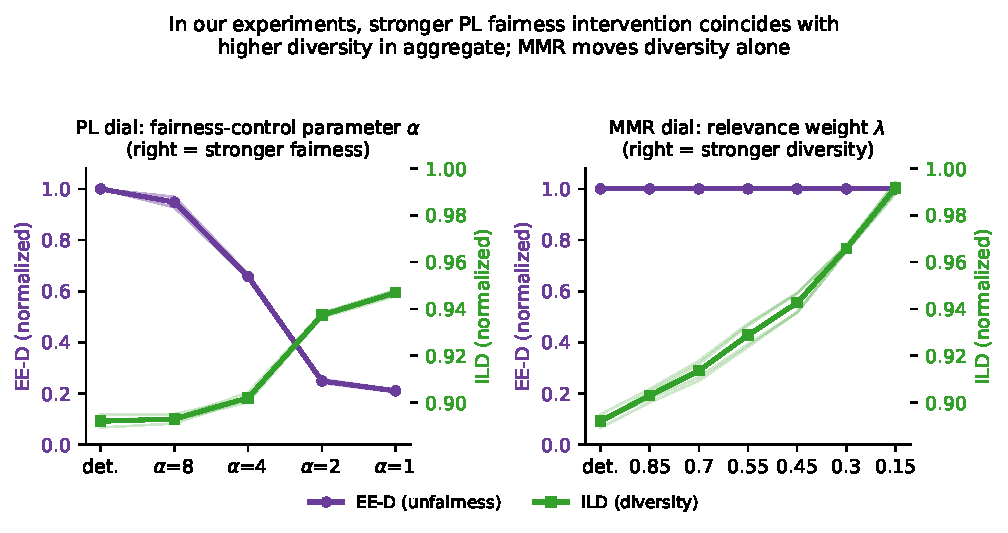
\includegraphics[width=0.92\textwidth]{fig2b_fairness_diversity_coupling.pdf}
\caption{In our experiments, stronger PL fairness intervention coincides
with higher diversity as an aggregate, by-$\alpha$ tendency (left panel):
PL's dial moves both expected exposure disparity and diversity at once.
This aggregate coupling is not tight at the level of individual queries
(row-level Pearson $r=-0.086$, Section~\ref{sec:premise}). MMR's dial
(right panel) moves diversity alone, with disparity pinned near the
deterministic level (EE-D $\approx 1$) and no explicit fairness
objective, which is what makes it usable as a diversity-focused
comparator against PL. Bold lines are the mean across the four
(generator, retriever) cells; thin lines are individual cells.}
\label{fig:premise}
\end{figure}

\FloatBarrier
\section{Results}
\label{sec:results}

\subsection{Finding 1: PL Reranking Generally Does Not Improve Utility}
\label{sec:finding1}

We test each PL $\alpha$ against the deterministic baseline, paired
per-query, Holm-corrected within each cell's 4-test family (4 $\alpha$
values $\times$ 4 generator/retriever cells $=16$ tests total). This
scopes the test specifically to PL, since MMR has no fairness objective
and does not belong in a test about whether fairness pays off; MMR-vs-baseline
comparisons are evidence about diversity instead
(Section~\ref{sec:finding3}).

Of the 16 tests, \textbf{10 are statistically significant, and 8 of those
are losses}. The two significant gains are both the same PL configuration
($\alpha=4$) in two different cells, and are small ($+0.0014$ and
$+0.0025$ in \eunorm{}) against losses roughly an order of magnitude
larger elsewhere.

Kim and Diaz's own reported result is more nuanced than ``fair rankings
often outperform'': they report an overall fairness/quality tradeoff in
which moderate fairness settings sometimes preserve or improve utility.
Given that our evaluation covers 2 of their 4 generators, 2 of their 3
retrievers, and $N=10$ sampled rankings against their $N=100$, we do not
frame this as contradicting their result outright. Within the two smaller
generators and two retrievers evaluated here, however, we do not
reproduce the pattern that moderate fair reranking frequently preserves or
improves deterministic-baseline utility: the direction is overwhelmingly
negative, with two small, real, but practically negligible exceptions.
Figure~\ref{fig:fig1} shows the deterministic baseline's normalized
utility across tasks and cells, illustrating the substantial cross-task
differences under our within-query normalization that motivate reporting
\eunorm{} rather than raw \eu{} throughout.

\begin{figure}[htbp]
\centering
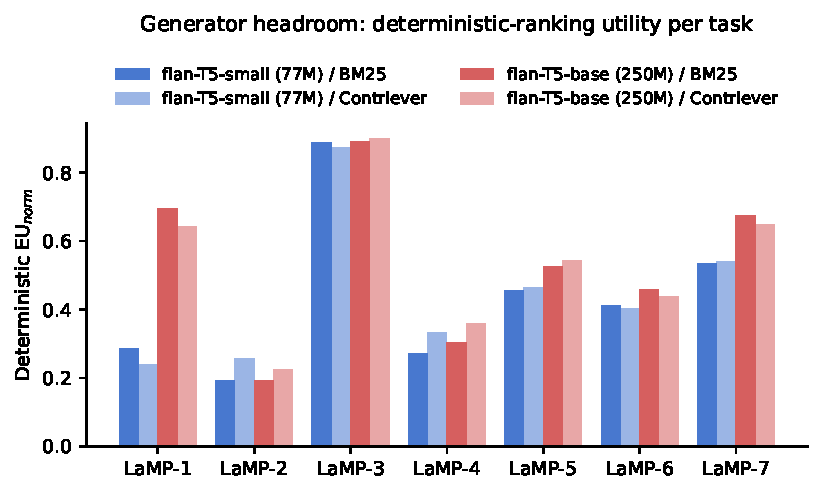
\includegraphics[width=0.85\textwidth]{fig1_headroom.pdf}
\caption{Deterministic-baseline normalized utility (\eunorm{}) by LaMP
task, for all four (generator, retriever) cells. \eunorm{} is each
query's raw utility divided by the largest raw utility it achieved across
its settings under that generator (Section~\ref{sec:normalization}), so
this figure shows the deterministic condition's relative performance
under that within-query normalization, not an absolute or task-independent
utility scale --- it illustrates why per-query normalization is necessary
for any cross-task comparison in this paper, not what generation quality
is achievable in some absolute sense.}
\label{fig:fig1}
\end{figure}

\subsection{Finding 2: A Real Fairness--Utility Tradeoff Within PL's Own Fairness Dial}
\label{sec:finding2}

We regress \eunorm{} on \eednorm{}, restricted to PL rows only, controlling
for \ildnorm{} and generator/retriever indicators:
\begin{multline}
\eunorm(q,s) = \beta_0 + \beta_1\,\eednorm(q,s) + \beta_2\,\ildnorm(q,s)
+ \beta_3\,\mathbf{1}\{\text{Base}\} + \beta_4\,\mathbf{1}\{\text{Contriever}\}
+ \varepsilon(q,s), \\ s \in \text{PL rows}.
\label{eq:finding2}
\end{multline}
Restricting to PL rows avoids mixing a within-method fairness manipulation
(PL's $\alpha$) with a between-method contrast (MMR and the deterministic
baseline sit at a fixed $\eed\approx1$ regardless of $\lambda$), which
would not be a clean fairness-dial estimate.

The primary estimate is $\hat\beta_1 = +0.0735$ (cluster-robust
$p=6.3\times10^{-54}$, $n=52{,}568$, 4{,}269 query clusters; the naive,
non-clustered $p=2.1\times10^{-93}$ overstates confidence by treating
repeated observations of the same query as independent). Because lower
\eed{} means fairer, a \emph{positive} coefficient means that
\textbf{less fair, more disparate rankings are associated with higher
utility} --- the opposite of what a ``fairness helps'' story would
predict.

\textbf{Robustness.} Leave-one-task-out, on the identical specification
and cluster-robust inference, keeps the coefficient positive and highly
significant under every single-task exclusion, ranging from $+0.0613$
(dropping LaMP-4, $p=1.9\times10^{-27}$) to $+0.0834$ (dropping LaMP-5,
$p=2.7\times10^{-53}$); no sign or significance flips. Query fixed effects
--- isolating the within-query association between \eednorm{} and
\eunorm{} from between-query composition --- give $+0.0518$
($p=2.0\times10^{-30}$); the finer query$\times$generator$\times$retriever
fixed effect, which isolates purely the $\alpha$-driven variation for one
exact query in one exact cell, gives $+0.0526$ ($p=2.4\times10^{-30}$),
essentially unchanged from the coarser fixed effect. The pooled estimate
was picking up some between-query variation, but the within-query
association remains substantial under every specification we tested
(Table~\ref{tab:fe-summary}).

\textbf{Task heterogeneity.} Fit on each task alone (no leave-one-task-out
exclusion, no other controls), the coefficient is positive in all seven
tasks, but not statistically significant on two of them in isolation
(LaMP-3, $p=0.31$; LaMP-7, $p=0.71$); the remaining five are individually
significant and positive. Unlike Findings 3 and 4, no task individually
reverses this association's sign. We nonetheless describe this as a
robust \emph{pooled} association rather than a claim that it is
statistically detectable within every single task in isolation, since two
of the seven do not reach significance on their own.

\begin{figure}[htbp]
\centering
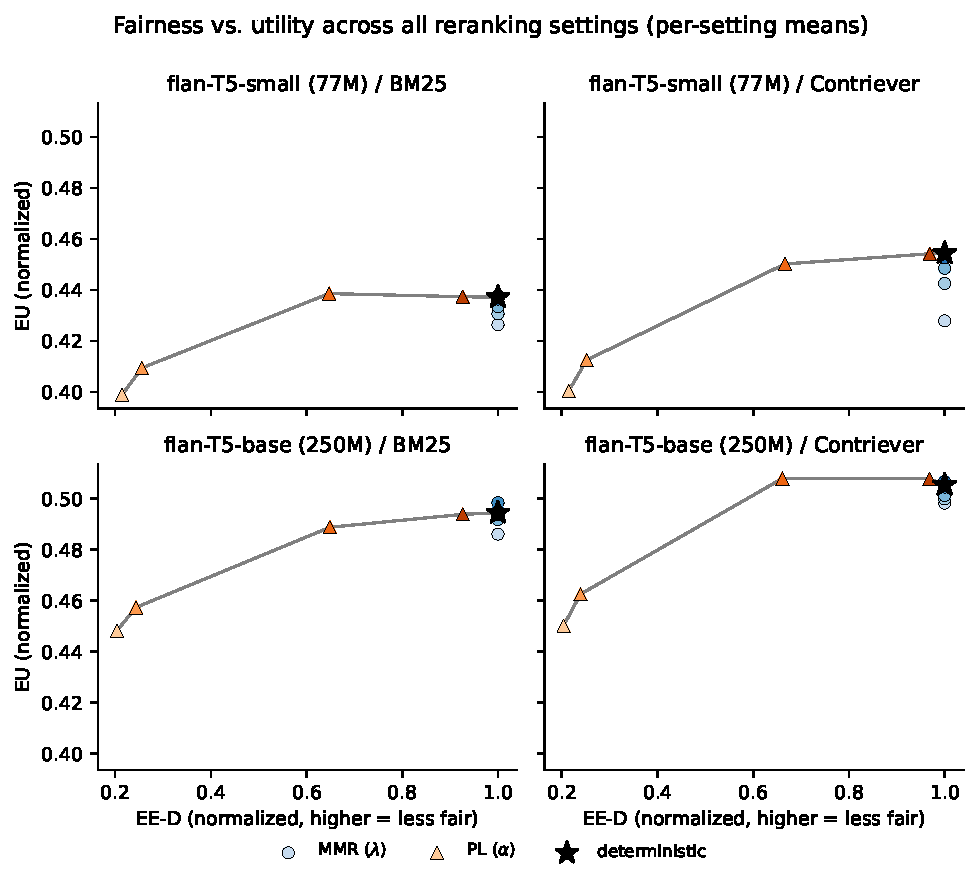
\includegraphics[width=0.92\textwidth]{fig2_fairness_utility_map.pdf}
\caption{Fairness (\eednorm{}, higher is less fair) versus utility
(\eunorm{}), per-setting means, one panel per generator/retriever cell.
PL's $\alpha$-trajectory is highlighted (triangles); MMR (circles) and the
deterministic baseline (star) are shown for context, but the Finding 2
regression (Eq.~\ref{eq:finding2}) uses PL rows only.}
\label{fig:fig2}
\end{figure}

\subsection{Finding 3: No General Utility Benefit From MMR Diversity}
\label{sec:finding3}

If measured within-list diversity were sufficient to explain any apparent
fairness benefit, diversity should help on its own, holding fairness
constant --- exactly what MMR, which has no fairness mechanism, lets us
test. We regress
\eunorm{} on \ildnorm{} within MMR rows only (exposure disparity is fixed
near the deterministic level, $\eed\approx1$, for all MMR settings):
\begin{multline}
\eunorm(q,s) = \gamma_0 + \gamma_1\,\ildnorm(q,s) + \gamma_2\,\mathbf{1}\{\text{Base}\}
+ \gamma_3\,\mathbf{1}\{\text{Contriever}\} + \varepsilon(q,s), \\ s \in \text{MMR rows}.
\label{eq:finding3}
\end{multline}

We find \textbf{no evidence of a general utility benefit from increased
MMR diversity}: the pooled association is modestly negative,
$\hat\gamma_1=-0.0675$ ($n=91{,}994$), cluster-robust $p=0.0115$ --- real,
but a considerably more modest significance level than the naive
$p=5.6\times10^{-10}$ suggested, since the repeated-query structure was
inflating confidence. We treat $p=0.0115$ as modest evidence for a real
modest negative association, not overwhelming evidence.

\textbf{Robustness.} The pooled coefficient stays negative under every
single-task exclusion (a sign check; no leave-one-task-out significance
claim is at stake here), but it does not hold in every task individually:
fit on LaMP-2 or LaMP-5 alone, the coefficient is positive. The pooled
negative association is robust to removing any one task, while the
direction itself is heterogeneous across tasks --- the diversity--utility
association is benchmark-dependent/heterogeneous across tasks, not a
fixed property of RAG generation. Query
fixed effects give $-0.0820$ ($p=2.4\times10^{-4}$), if anything larger in
magnitude than the pooled estimate; the finer
query$\times$generator$\times$retriever fixed effect gives $-0.0785$
($p=5.0\times10^{-4}$), essentially unchanged (Table~\ref{tab:fe-summary}).

\textbf{Per-cell heterogeneity.} Figure~\ref{fig:fig4} and
Table~\ref{tab:percell} report the identical bivariate specification
(\ildnorm{} only, no controls) fit separately within each cell, with
cluster-robust inference. Only the Flan-T5-Base/BM25 cell is individually
significant. A formal test of whether the visually larger Base-cell
coefficients reflect a genuine generator-size interaction --- a pooled
within-MMR regression with an \ildnorm{}$\times$generator interaction
term, cluster-robust by query and controlling for task and retriever ---
gives $p=0.28$: not significant. The descriptive per-cell pattern in
Figure~\ref{fig:fig4} is real and visible, but the formal test does not
confirm generator size as its driver.

\begin{table}[htbp]
\centering
\caption{Per-cell bivariate regression of \eunorm{} on \ildnorm{} within
MMR rows (no controls), matching Figure~\ref{fig:fig4} exactly.}
\label{tab:percell}
\begin{tabular}{lrl}
\toprule
Cell & Coefficient & $p$ \\
\midrule
Flan-T5-Small / BM25 & $-0.0374$ & $0.34$ \\
Flan-T5-Small / Contriever & $-0.0149$ & $0.69$ \\
Flan-T5-Base / BM25 & $-0.1483$ & $8.9\times10^{-5}$ \\
Flan-T5-Base / Contriever & $-0.0728$ & $0.068$ \\
\bottomrule
\end{tabular}
\end{table}

\begin{figure}[htbp]
\centering
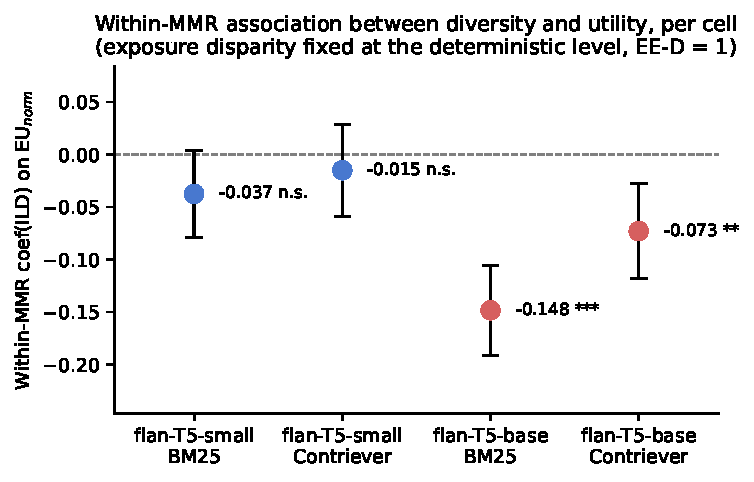
\includegraphics[width=0.72\textwidth]{fig4_ild_signflip.pdf}
\caption{Within-MMR association between diversity and utility, per cell,
with exposure disparity fixed at the deterministic level. Coefficients
correspond to Table~\ref{tab:percell}.}
\label{fig:fig4}
\end{figure}

\textbf{Direct MMR-vs-deterministic comparison.} As a complementary,
non-regression check, we test whether MMR ever significantly beats or
loses to the deterministic baseline directly: paired per-query, all
$7\;\lambda$ values $\times\;4$ cells $=28$ comparisons (every MMR setting
run, not a pre-selected subset), Holm-corrected within each cell's 7-test
family. \textbf{4 of 28 are significant, and all 4 are losses}
(Table~\ref{tab:mmr-vs-det}). The pattern is consistent with the negative
diversity--utility association above (lower $\lambda$ trades more
relevance for more diversity, not diversity in isolation, so this is not
independent confirmation of a diversity-specific effect): every
significant loss occurs at the two strongest-diversity settings, and the
per-cell delta shrinks toward zero monotonically as $\lambda\to1$, where
it is exactly 0.0 in every cell by the construction check of
Section~\ref{sec:setup}. Overall, 19 of 28 comparisons point negative, and
MMR shows no significant utility \emph{win} over the deterministic
baseline in any of the 28 settings tested.

\begin{table}[htbp]
\centering
\caption{MMR versus deterministic baseline, paired per-query, aggregated
over the four generator/retriever cells (28 comparisons total,
Holm-corrected within each cell's 7-test family).}
\label{tab:mmr-vs-det}
\begin{tabular}{lrr}
\toprule
MMR $\lambda$ & Cells with negative $\Delta$ (of 4) & Cells significant (of 4) \\
\midrule
0.15 & 4 & 3 \\
0.30 & 4 & 1 \\
0.45 & 4 & 0 \\
0.55 & 2 & 0 \\
0.70 & 3 & 0 \\
0.85 & 2 & 0 \\
1.00 & 0 (exactly zero, by construction) & 0 \\
\bottomrule
\end{tabular}
\end{table}

\subsection{Finding 4: A Residual PL--MMR Utility Difference After Adjusting for Diversity}
\label{sec:finding4}

Restricting to PL and MMR rows, we ask whether being a PL setting (versus
MMR) predicts a further utility difference once measured diversity is
accounted for. This is a regression adjustment, not a matching procedure.

\textbf{Additive specification.} Table~\ref{tab:finding4-additive}
reports the per-cell coefficient of a PL indicator on \eunorm{},
controlling for \ildnorm{}; all four cells are negative, significant, and
of similar magnitude. Pooling with a single common \ildnorm{} slope for PL
and MMR gives an additive PL-indicator coefficient of $-0.0194$
(cluster-robust $p=8.8\times10^{-34}$) --- but before treating this single
number as the answer, we test whether a single common slope is the right
model.

\begin{table}[htbp]
\centering
\caption{Per-cell coefficient of the PL indicator on \eunorm{}, controlling
for \ildnorm{} (additive specification).}
\label{tab:finding4-additive}
\begin{tabular}{lrl}
\toprule
Cell & Coefficient & $p$ (cluster-robust) \\
\midrule
Flan-T5-Small / BM25 & $-0.0130$ & $1.1\times10^{-7}$ \\
Flan-T5-Base / BM25 & $-0.0226$ & $5.5\times10^{-17}$ \\
Flan-T5-Small / Contriever & $-0.0186$ & $1.4\times10^{-12}$ \\
Flan-T5-Base / Contriever & $-0.0227$ & $1.9\times10^{-16}$ \\
\bottomrule
\end{tabular}
\end{table}

\textbf{Primary specification: does the gap depend on diversity level?}
We add a PL$\times$\ildnorm{} interaction term:
\begin{multline}
\eunorm(q,s) = \beta_0 + \beta_1\,\isPL(s) + \beta_2\,\ildnorm(q,s) \\
+ \beta_3\,\big(\isPL(s)\times\ildnorm(q,s)\big)
+ \beta_4\,\mathbf{1}\{\text{Base}\} + \beta_5\,\mathbf{1}\{\text{Contriever}\}
+ \textstyle\sum_t \beta_t\,\mathbf{1}\{\text{task}=t\} + \varepsilon(q,s).
\label{eq:finding4-interaction}
\end{multline}
Controls are a generator indicator, a retriever indicator, and LaMP-task
fixed effects, matching every other pooled specification in this paper;
inference is cluster-robust by query (CR1 sandwich estimator), and
Table~\ref{tab:finding4-additive}'s per-cell $p$-values use this same
cluster-robust inference, not classical standard errors. The interaction
is significant in the pooled specification
($\hat\beta_3=+0.0293$, $p=0.0125$): the two methods' \ildnorm{} slopes
are not identical, so a single additive coefficient understates what is
happening. Because \ildnorm{} is not centered, $\hat\beta_1$ alone is the
model's fitted PL--MMR gap specifically at $\ildnorm=0$; that value does
occur in the data (both methods' observed \ildnorm{} minimum is exactly
0.0) but is rare, since \ildnorm{}'s own 10th percentile is already 0.84.
Table~\ref{tab:finding4-conditional} reports the conditional gap,
$\Delta(\ildnorm)=\hat\beta_1+\hat\beta_3\cdot\ildnorm$, at several points
across the observed range, together with the average marginal effect
(AME), the same quantity evaluated at the empirical mean of \ildnorm{}.

\begin{table}[htbp]
\centering
\caption{Conditional PL--MMR gap at points across the observed \ildnorm{}
range, and the average marginal effect (AME), from the interaction model
(Eq.~\ref{eq:finding4-interaction}).}
\label{tab:finding4-conditional}
\begin{tabular}{lrrr}
\toprule
\ildnorm{} level & $\Delta$(PL$-$MMR) & 95\% CI & $p$ \\
\midrule
0 (observed floor, rare) & $-0.0464$ & $[-0.068,\,-0.025]$ & $2.1\times10^{-5}$ \\
$p_{10}$ (0.84) & $-0.0218$ & $[-0.025,\,-0.018]$ & $2.5\times10^{-32}$ \\
median (0.96) & $-0.0181$ & $[-0.021,\,-0.015]$ & $2.8\times10^{-27}$ \\
$p_{90}$ (0.99) & $-0.0172$ & $[-0.021,\,-0.014]$ & $3.6\times10^{-21}$ \\
\textbf{mean (AME)} & \textbf{$-0.0192$} & \textbf{$[-0.022,\,-0.016]$} & \textbf{$1.5\times10^{-33}$} \\
\bottomrule
\end{tabular}
\end{table}

The gap is largest, about $-0.046$, in the small, rare tail of
low-diversity settings, and narrows to roughly $-0.017$ to $-0.022$ across
the bulk of the data ($p_{10}$ to $p_{90}$ of observed \ildnorm{}). We
treat the AME, $-0.0192$, as the headline single-number summary of
Finding 4: a proper average over the interaction model rather than an
assumption of one fixed slope, and it lands almost exactly where the
simpler additive coefficient ($-0.0194$) did.

\textbf{Is the interaction itself robust?} Not entirely, though the AME
built from it is. Under the strictest identification we use ---
query$\times$generator$\times$retriever fixed effects --- the interaction
shrinks and loses significance ($\hat\beta_3=+0.0157$, $p=0.15$), about
half the pooled magnitude and no longer distinguishable from zero.
Leave-one-task-out on the pooled interaction model keeps the coefficient
positive when 6 of 7 tasks are dropped individually (range $+0.023$ to
$+0.037$; five of those six drops are individually significant, $p$ from
$0.003$ to $0.021$, and the sixth, dropping LaMP-7, is not, $p=0.061$),
but \textbf{flips sign when LaMP-6 is dropped} ($-0.0280$, $p=0.16$, itself
not significant either way) --- the only one of the seven folds to do so. We therefore treat the diversity-dependence
pattern --- the interaction term itself --- as a suggestive, secondary
observation, not an established one. What \emph{does} survive, robustly,
across every specification we tried (pooled, query fixed effects,
query$\times$generator$\times$retriever fixed effects, and all seven
leave-one-task-out folds) is the AME itself: it ranges narrowly from
$-0.0161$ to $-0.0217$ across every leave-one-task-out fold (all
$p<10^{-17}$), and from $-0.0192$ to $-0.0200$ across the pooled and
fixed-effects variants (Table~\ref{tab:fe-summary}), always
highly significant and never close to flipping sign. Figure~\ref{fig:fig7}
shows the raw per-quintile pattern that motivates the interaction check;
we caution against reading the apparent low-vs-high-diversity gap in that
figure as an established, robust pattern in its own right --- it is the
AME in Table~\ref{tab:fe-summary}, not the bin-level shape of
Figure~\ref{fig:fig7}, that is the robust quantity.

\textbf{What this does and does not establish.} Adjusting for \ildnorm{}
controls for one measured outcome of the ranking, not for everything that
differs between PL and MMR: PL is stochastic and MMR deterministic, the
two methods may preserve the underlying relevance ordering differently,
and PL introduces variance across repeated draws that MMR does not have.
The AME is therefore an \emph{average adjusted difference} between PL and
MMR after controlling for measured \ildnorm{}, not a causal estimate of
what fairness itself costs.

\textbf{Common support.} Does the comparison rely on extrapolating outside
the diversity range either method actually reaches? No: PL's and MMR's
measured \ildnorm{} distributions essentially fully overlap (closely
aligned 5th/median/95th percentiles), and restricting to their common
support changes nothing: the secondary additive PL-indicator coefficient
is $-0.0193$ ($p=8.8\times10^{-34}$; all 144{,}562 rows already fall
inside the overlap) --- the interaction-model AME above is grounded in the
full sample, unaffected by this restriction.

\textbf{Mechanism test.} We hypothesized that PL pays a \emph{relevance}
cost --- stochastic sampling moves away from the highest-ranked item, and
that specifically, not diversity, explains the residual. \eer{} is a
direct proxy for exposure-relevance alignment. In this secondary additive
mechanism-check specification, adding \eernorm{} as a covariate moves the
PL-indicator coefficient from $-0.0194$ to $-0.0187$
($p=3.0\times10^{-34}$) --- essentially unchanged, even though \eernorm{}
itself is strongly associated with utility on its own
($\hat\beta=+0.158$, $p=5.1\times10^{-104}$, a sanity check that \eernorm{}
behaves as expected). \textbf{This relevance-cost hypothesis is not
confirmed by the test.} PL underperforms MMR on average after adjusting
for \ildnorm{}, robustly across the specifications tested; the pooled
interaction model suggests a larger disadvantage in the rare
low-diversity tail, but that interaction does not survive the strictest
fixed-effects and leave-one-task-out checks, and the residual mechanism
remains unidentified. It may relate to the stochasticity itself (variance,
not just a mean shift) or to some other ranking property that \ildnorm{}
and \eernorm{} together do not capture, but the present experiment does
not identify which. Supplementary Figure~\ref{fig:fig5} (Appendix~\ref{app:supp})
provides the corresponding per-task descriptive PL--MMR differences within
shared ILD bins; we present it as descriptive detail underlying the AME
above, not as independent robustness evidence.

\begin{figure}[htbp]
\centering
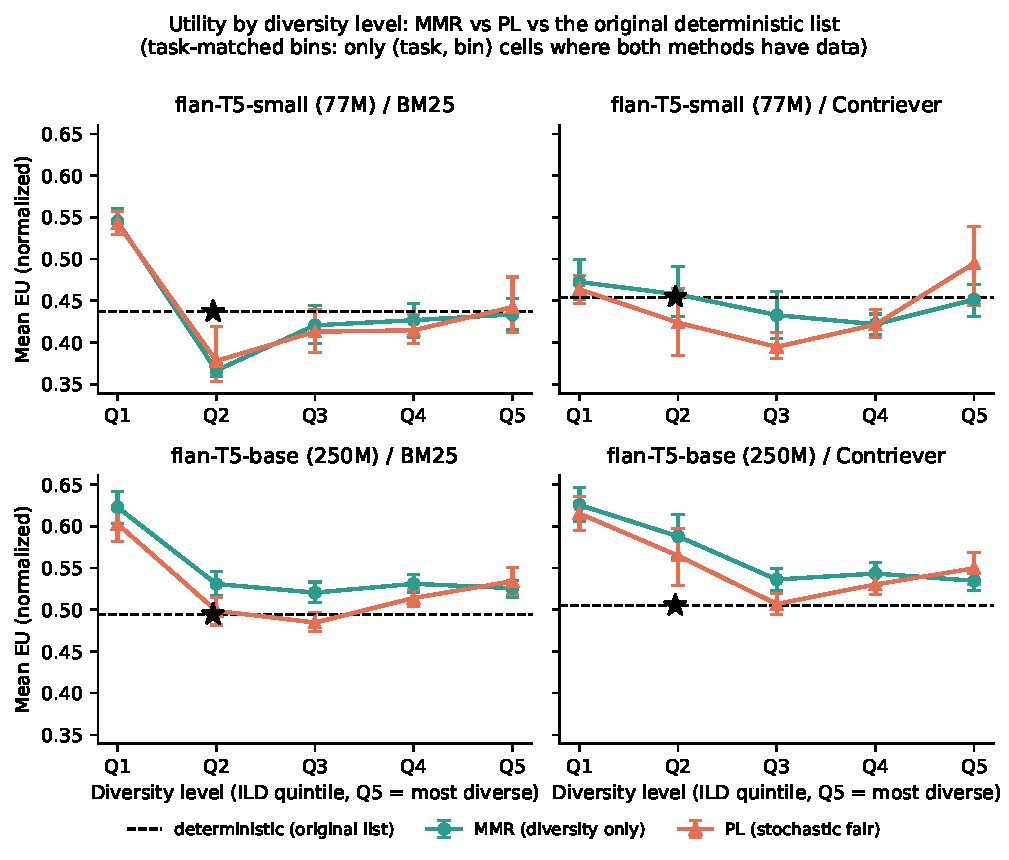
\includegraphics[width=0.92\textwidth]{fig7_eu_by_diversity_level.pdf}
\caption{Mean utility by diversity quintile, MMR versus PL, with the
deterministic baseline shown for reference. Error bars are 95\% confidence
intervals from a task-stratified bootstrap (400 resamples, each task
resampled with replacement and averaged with equal task weight, 2.5th/
97.5th percentiles). This raw, descriptive pattern motivated the
interaction check of Table~\ref{tab:finding4-conditional}; as discussed in
the text, the AME is the robust summary of Finding 4, not the specific
low-vs-high quintile shape visible here.}
\label{fig:fig7}
\end{figure}

\FloatBarrier
\section{Robustness Analyses}
\label{sec:robustness}

\textbf{Leave-one-task-out.} The headline pooled coefficients for
Findings 2 and 3 were checked leave-one-task-out; neither's main
conclusion depends on any single task remaining in the sample. Finding 4's
AME is similarly leave-one-task-out robust (every fold $-0.016$ to
$-0.022$, always significant), while the PL$\times$\ildnorm{} interaction
underlying its secondary diversity-dependence framing is not (it flips
sign when LaMP-6 is dropped). This does not cover every secondary
specification in this paper (per-cell regressions, the generator
interaction, the \eer{} mechanism check); those were not individually
re-run leave-one-task-out.

\textbf{Cluster-robust inference.} Added throughout to correct for
repeated observations of the same query across settings; it changes exact
significance levels (most notably Finding 3, where the naive
$p=5.6\times10^{-10}$ becomes $p=0.0115$ once clustering is applied) but
does not overturn any finding's direction or overall conclusion.

\textbf{Fixed effects.} Table~\ref{tab:fe-summary} summarizes all three
findings under query fixed effects and the finer
query$\times$generator$\times$retriever fixed effect. For Finding 4, we
report the AME from the interaction model at each fixed-effects level
(not the additive coefficient) as the headline robustness quantity, per
the primary specification of Section~\ref{sec:finding4}; the additive
coefficient (also fixed-effects-robust, at $-0.0200$ under both levels) is
a secondary check. The two fixed-effects levels barely differ from each
other for any finding, indicating that cell composition was not doing
hidden work in the coarser, query-only version.

\begin{table}[htbp]
\centering
\caption{Pooled coefficients versus query fixed effects and the finer
query$\times$generator$\times$retriever fixed effect. Finding 4's row
reports the AME from the interaction model (Eq.~\ref{eq:finding4-interaction}),
not the additive coefficient, consistent with Section~\ref{sec:finding4}.}
\label{tab:fe-summary}
\small
\begin{tabular}{lccc}
\toprule
Finding & Pooled & Query FE & Query$\times$gen.$\times$retr.\ FE \\
\midrule
2 (coef.\ \eed{}, PL rows) & $+0.0735$ & $+0.0518$ & $+0.0526$ \\
 & ($p=6.3\times10^{-54}$) & ($p=2.0\times10^{-30}$) & ($p=2.4\times10^{-30}$) \\
3 (coef.\ \ild{}, MMR rows) & $-0.0675$ & $-0.0820$ & $-0.0785$ \\
 & ($p=0.0115$) & ($p=2.4\times10^{-4}$) & ($p=5.0\times10^{-4}$) \\
4 (AME, PL+MMR) & $-0.0192$ & $-0.0200$ & $-0.0200$ \\
 & ($p=1.5\times10^{-33}$) & ($p=1.6\times10^{-36}$) & ($p=2.0\times10^{-36}$) \\
\bottomrule
\end{tabular}
\end{table}

\textbf{Normalization sensitivity.} As described in
Section~\ref{sec:normalization}, filling the 3.5\% of rows excluded by the
zero-denominator condition, rather than dropping them, leaves all three
conclusions unchanged.

\textbf{Task-robustness figure.} Figure~\ref{fig:fig8} visualizes the
leave-one-task-out check for Findings 2 and 3's pooled coefficients
together, each on its exact final specification (Finding 2: PL rows only;
Finding 3: MMR rows only); both retain their sign and significance status
under every single-task exclusion. Finding 4's leave-one-task-out
robustness is reported separately in Section~\ref{sec:finding4} and
Table~\ref{tab:fe-summary}, since its headline quantity (the
interaction-model AME) is not a single additive coefficient this
panel layout can show alongside Findings 2--3 without visually implying
the fragile PL$\times$\ildnorm{} interaction is itself the headline
result.

\begin{figure}[htbp]
\centering
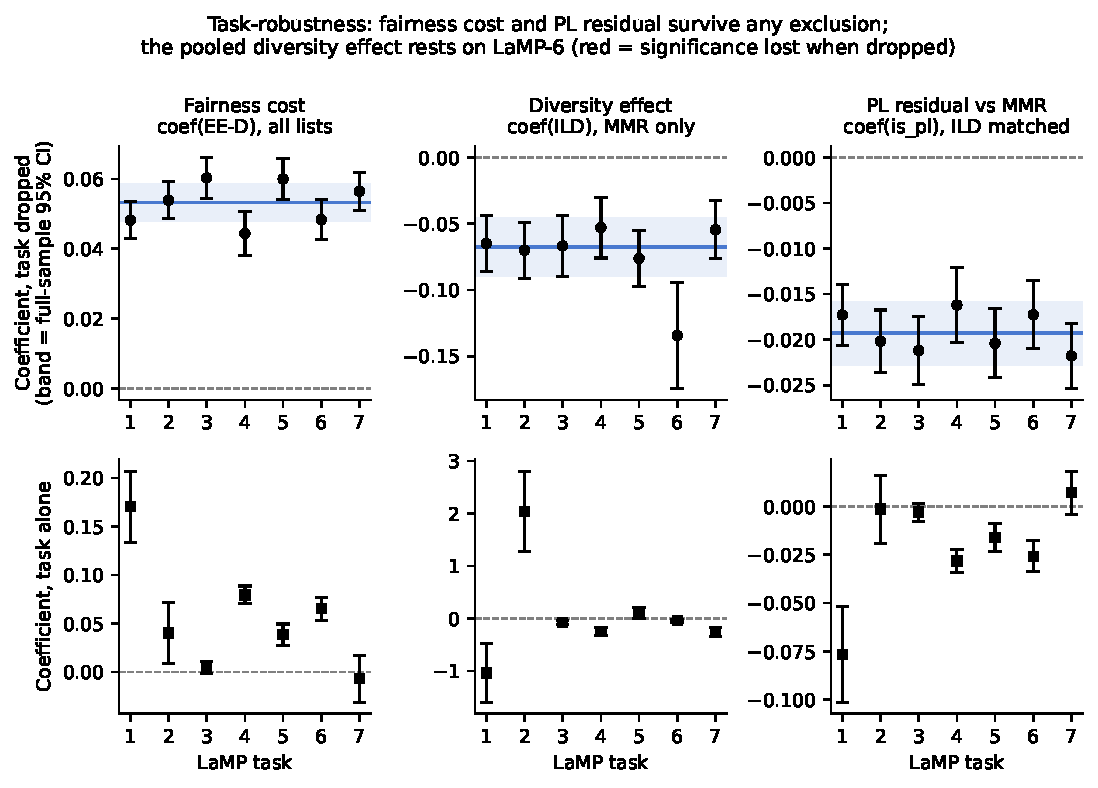
\includegraphics[width=0.8\textwidth]{fig8_task_sensitivity.pdf}
\caption{Leave-one-task-out robustness for Findings 2 and 3's pooled
coefficients. Top row: coefficient when each task is dropped, against the
full-sample estimate (blue band, 95\% CI). Bottom row: coefficient fit on
each task alone --- Finding 2 (left) is positive in every task alone,
though not statistically significant in two of them; Finding 3 (right)
reverses sign in two tasks fit alone. No task exclusion flips the sign or
significance status of either pooled coefficient.}
\label{fig:fig8}
\end{figure}

\FloatBarrier
\section{Discussion}
\label{sec:discussion}

This paper set out to answer a specific question: when fair reranking
appears to help or hurt RAG generation quality, is that attributable to
fairness itself, or to the within-list diversity the fairness mechanism
happens to induce? Across the settings we test, the answer is that
\textbf{measured within-list diversity (ILD-Jaccard) alone does not
account for the difference between PL and MMR utility}. PL's own
fairness dial is associated with a real, robust, and negative
relationship to utility (Finding 2); MMR's diversity dial shows no general
utility benefit of its own, and if anything a modest negative association
(Finding 3); and PL retains an average utility disadvantage relative to
MMR even after adjusting for measured diversity (Finding 4). If measured
ILD-Jaccard were sufficient to explain PL's apparent utility behavior, we
would expect the diversity variation MMR induces in that measured quantity
to show a corresponding general utility benefit on its own; we do not
observe such a pattern.

This is a narrower conclusion than Kim and Diaz's original finding might
suggest, but the two results are not necessarily in tension: our
evaluation covers 2 of their 4 generators, 2 of their 3 retrievers, and a
tenfold-lower PL sample count ($N=10$ versus $N=100$), and we do not claim
to have reproduced their full experimental grid. What we can say is that,
within the Flan-T5-Small and Flan-T5-Base, BM25 and Contriever setting we
do test, fair reranking does not reproduce the pattern of frequently
preserving or improving utility, and that the diversity-as-mechanism
hypothesis specifically does not explain the residual gap between the two
reranking families.

It is important to be precise about what the PL-vs-MMR comparison in
Finding 4 does and does not identify. Because PL and MMR differ along
several dimensions besides measured diversity --- stochastic sampling
versus deterministic selection, and how each method preserves or disturbs
the underlying relevance ordering, among others --- the residual utility
gap after adjusting for \ildnorm{} is an \emph{adjusted association}, not
a causal estimate of what fairness itself costs. We tested the most
obvious candidate explanation directly: that PL's randomization imposes a
relevance cost, measurable via exposure-relevance alignment (\eer{}).
Adding \eer{} as a covariate left the residual essentially unchanged,
so this specific mechanism is not confirmed. The residual mechanism
remains unidentified; it may relate to the variance PL's stochastic
sampling introduces, rather than only its mean shift, or to some property
of the ranking that neither \ildnorm{} nor \eernorm{} captures, but this
remains an open question for future work, which we discuss should require
a design that varies fairness and diversity independently rather than
only adjusting for one while measuring the other.

Finally, task heterogeneity recurs throughout, though not always as a sign
reversal: Finding 2's association is positive in all seven tasks fit
alone but not statistically distinguishable from zero in two of them
(LaMP-3, LaMP-7); Finding 3's association reverses sign on LaMP-2 and
LaMP-5 alone; Finding 4's secondary diversity-dependence interaction
reverses sign when LaMP-6 is excluded. None of these task-level patterns
overturn the corresponding pooled, leave-one-task-out-robust conclusion,
but they
are a reminder that these associations are properties of a
query-weighted pool of seven quite different personalization tasks, not
of RAG generation in general.

\section{Limitations}
\label{sec:limitations}

\begin{itemize}
\item \textbf{Generator scale.} We evaluate only Flan-T5-Small (77M) and
  Flan-T5-Base (250M). Whether this tradeoff grows, shrinks, or reverses
  at larger generator scales is untested here; utility labels exist for a
  much larger (XXL) generator in the source release, but it does not fit
  the GPU hardware available for this project.
\item \textbf{Retriever coverage.} We evaluate BM25 and Contriever only,
  2 of the 3 retrievers in the source paper's evaluation.
\item \textbf{PL sample count.} $N=10$ sampled rankings per $(q,\alpha)$
  pair, against the source paper's $N=100$; our PL-based \eed{}/\eu{}
  estimates carry more Monte Carlo noise than theirs. A cheap follow-up
  --- recomputing \eed{} only at $N=100$ on a subset, without regenerating
  text --- would quantify Monte Carlo sensitivity of the exposure metrics
  specifically, but would not by itself bound Monte Carlo uncertainty in
  generated utility; this was not run for this paper.
\item \textbf{Diversity operationalization.} We measure diversity as
  ILD-Jaccard, a single specific notion of within-list textual variety;
  our conclusion that measured diversity does not account for the
  PL--MMR gap is a claim about \emph{this} operationalization, not about
  every possible notion of diversity.
\item \textbf{Loose fairness--diversity coupling.} \eed{} and \ild{} are
  conceptually distinct quantities that are only loosely, not strictly,
  coupled under PL in this data (Section~\ref{sec:premise}); this limits
  how cleanly any \ildnorm{}-adjusted comparison can isolate fairness's
  own contribution.
\item \textbf{PL and MMR differ beyond diversity.} PL is stochastic and
  MMR deterministic; the two methods may preserve the original relevance
  ordering differently, and only PL introduces sampling variance across
  repeated draws. Finding 4's residual should not be read as an isolated
  measurement of fairness's causal effect for this reason.
\item \textbf{Task dependence.} Findings 2 and 3's pooled effects are
  leave-one-task-out robust. Finding 2's association is positive in every
  task fit alone, though not statistically significant in two of them
  (LaMP-3, LaMP-7); Finding 3's association does reverse sign on two
  tasks fit alone (LaMP-2, LaMP-5). Finding 4's AME is similarly robust,
  but the interaction term underlying its secondary
  diversity-dependence framing is not (it loses significance under the
  strictest fixed effects and flips sign when LaMP-6 is dropped); we
  treat that pattern as secondary for exactly this reason.
\end{itemize}

\section{Conclusion}
\label{sec:conclusion}

We asked whether an apparent fairness benefit in RAG generation quality is
attributable to fairness itself or to the within-list diversity that a
fairness mechanism happens to induce. Using all available queries retained
by Kim and Diaz's generator-specific fairness-evaluation collections
across all seven LaMP tasks, two generators, and two retrievers, we find
that PL
fair reranking does not generally improve utility over a deterministic
baseline; that within PL's own fairness dial, greater exposure equality is
robustly associated with lower utility; that MMR's explicit diversity dial
shows no general utility benefit on its own; and that PL retains an
average utility disadvantage relative to MMR even after adjusting for
measured diversity, a disadvantage that a direct test of a relevance-cost
mechanism does not explain. Taken together, \textbf{measured within-list
diversity (ILD-Jaccard) alone does not account for the PL--MMR utility
difference} we observe, while the residual itself should not be read as
the isolated causal cost of fairness, since PL and MMR differ along
dimensions besides diversity. Determining what does explain that residual
--- and whether these patterns persist at larger generator scale and
across additional retrievers --- is the natural next step, and would
benefit from an experimental design that varies fairness and diversity
independently rather than adjusting for one while measuring the other.

\bibliographystyle{plainnat}
\bibliography{references}

\clearpage
\appendix
\section{Supplementary Figure}
\label{app:supp}

\begin{figure}[H]
\centering
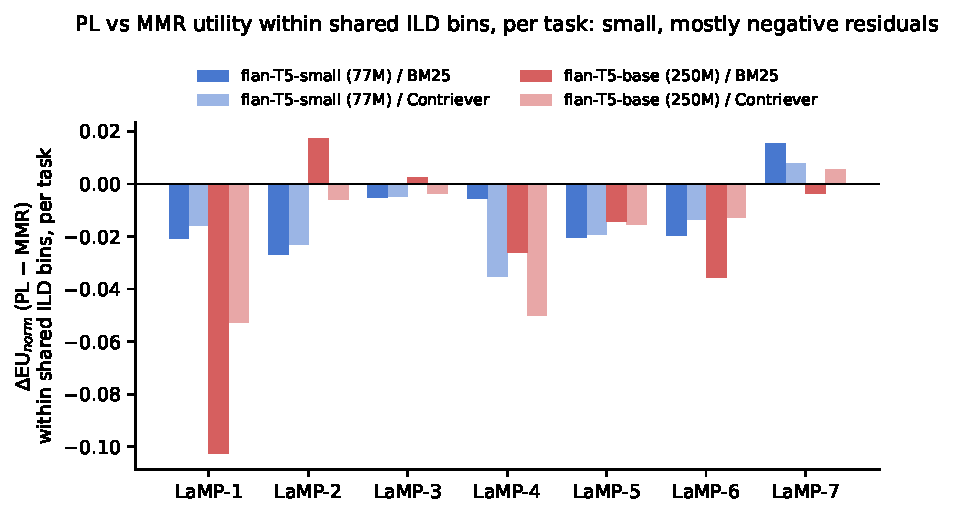
\includegraphics[width=0.95\textwidth]{fig5_matched_diversity.pdf}
\caption{Per-task detail underlying Finding 4: mean \eunorm{} difference
(PL minus MMR) within shared ILD bins --- a descriptive binned
comparison, not a formal statistical matching procedure --- by LaMP task
and generator/retriever cell. Residuals are small and mostly negative,
consistent with the pooled AME of Section~\ref{sec:finding4}; this
per-task breakdown is supplementary detail, not an independent robustness
claim.}
\label{fig:fig5}
\end{figure}

\end{document}
